\documentclass[a4paper,12pt,twoside]{memoir}
\usepackage{longtable}
\usepackage{btp}    % Use the trainermanual package option (i.e. \usepackage[trainermanual]{btp}) to generate the Trainer's version of the manual
%\usepackage[
%  noinfo,
%  cam,
%  cross,                % crosses as marks
%  a4,
%  width=6.25in,         % the width of the galley
%  height=9.25in,        % the height of the galley
%  center                % actual page is centered on the galley
%]{crop}
% Set some Workshop specific info

%\usepackage{underscore}

\usepackage{color}
\definecolor{light-blue}{rgb}{0.8,0.85,1}


\setWorkshopTitle{Introduction to Command-Line \\[5mm]
					\& Scripting For Bioinformatics}
\setWorkshopVenue{University of Adelaide}
\setWorkshopDate{24th March, 2016}
\setWorkshopAuthor{
Steve Pederson\\
Stephen Bent\\
Dan Kortschak\\
}
\begin{document}

%
% Workshop Title Page
%
\workshoptitlepage

%
% CC-BY
%
\input{licences/licence.tex}
\clearpage

\tableofcontents

\chapter{Workshop Information}
\clearpage

%
% Trainers Page
%
\section{The Trainers}

\newlength{\trainerIconWidth}
\setlength{\trainerIconWidth}{2.0cm}

\begin{center}
\begin{longtable}{>{\centering\arraybackslash} m{1.1\trainerIconWidth} m{1\textwidth}}

  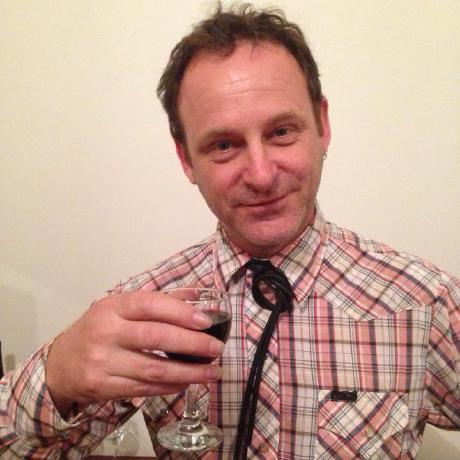
\includegraphics[width=\trainerIconWidth]{photos/steveped.jpeg} &
    \textbf{Mr. Steve Pederson}\newline
    Co-ordinator\newline
    Bioinformatics Hub\newline
    The University of Adelaide\newline
    South Australia\newline
    \mailto{stephen.pederson@adelaide.edu.au}\\
    \\
    
  
\includegraphics[width=\trainerIconWidth]{photos/jimmyb.png} &
    \textbf{Dr. Jimmy Breen}\newline
    Bioinformatician\newline
    Bioinformatics Hub \& Robinson Research Institure\newline
    The University of Adelaide\newline
    South Australia\newline
    \mailto{jimmy.breen@adelaide.edu.au}\\
    \\
  
\includegraphics[width=\trainerIconWidth]{photos/hien.png} &
    \textbf{Dr. Hien To}\newline
    Bioinformatician\newline
    Bioinformatics Hub\newline
    The University of Adelaide\newline
    South Australia\newline
    \mailto{hien.to@adelaide.edu.au}\\
  
  
\end{longtable}
\end{center}



%
% Workshop Preamble
%
%
% Start: General Information describing the workshop and the structure of the handouts
%
\newpage
\section{Welcome}
Thank you for your attendance \& welcome to the Introduction to Command Line \& Shell Scripting Workshop.
This is an offering by the University of Adelaide, Bioinformatics Hub which is a centrally funded initiative from the Department of Vice-Chancellor (Research), with the aim of assisting \& enabling researchers in their work.
Training workshops \& seminars such as this one  are an important part of this initiative. 
The Bioinformatics Hub itself has a web-page at \url{http://www.adelaide.edu.au/bioinformatics-hub/}, and to be kept up to date on upcoming events and workshops, please join the internal Bioinformatics mailing list on \url{http://list.adelaide.edu.au/mailman/listinfo/bioinfo}.\\

The Bioinformatics Hub has just started a Twitter account, so please follow us on (\url{https://twitter.com/UofABioinfoHub/}).
We also have an active Slack team for discussing Bioinformatics questions with the local community.
Slack teams do require an invitation to join, so please email the Hub on \mailto{bioinf_hub@adelaide.edu.au} to join the community.
All are welcome.\\

Today's workshop has been put together based on previous material and courses prepared by Dr Stephen Bent (\textit{University of Queensland}), with generous technical support \& advice provided by Dr Nathan Watson-Haigh (\textit{ACPFG}) and Dr Dan Kortschak (\textit{Adelaide University, Adelson Research Group}). 
We hope it will be useful in enabling you to continue and to advance your research.\\

\section{Course Summary}
In today's workshop, the morning session will be spent introducing you to the basic tools and concepts required for data handling.
In the afternoon session we'll develop these skills to a more advanced level, with progress in both sessions being made at your own pace.
Some people may finish early today, but the majority of you probably won't.
The VMs you use will be active for the next few weeks should you wish to continue working through the material after the workshop \\

The majority of data handling and analysis required in the field of bioinformatics uses the \textit{command line}, alternatively known as the terminal or the \textit{bash shell}.
This is a text-based interface in which commands must be typed, as opposed to the Graphical User Interfaces (aka GUIs) that most of us have become accustomed to.
Being able to access your computer using these tools enables you to more fully utilise the power \& capabilities of your machine, for both Linux \& Mac operating systems, and to a lesser extent will even enable you to dig deeper on a Windows system.\\

Whilst some of the tools we cover today may appear trivial, they will be used on a daily basis once you begin working in the field.
These basic tools will also be very useful for writing what are known as \textit{shell scripts}, which we will begin to cover in the afternoon session.
These are essentially simple programs that utilise the inbuilt functions of the shell, and are used to automate processes such as de-multiplexing read libraries, or aligning reads to the genome.
A knowledge of this simple type of programming is also essential for accessing the high-performance computing resources as offered by eResearch SA (\url{www.ersa.edu.au}).


\section{Providing Feedback}
While we endeavour to deliver a workshop with quality content and documentation in a venue conducive to an exciting, well run hands-on workshop with a bunch of knowledgeable and likable
trainers, we know there are things we could do better.

Whilst we want to know what didn't quite hit the mark for you, what would be most helpful and least
depressing, would be for you to provide ways to improve the workshop. i.e. constructive feedback.
After all, if we knew something wasn't going to work, we wouldn't have done it or put it into the
workshop in the first place!

Clearly, we also want to know what we did well! This gives us that ``feel good'' factor which will
see us through those long days and nights in the lead up to such hands-on workshops!

With that in mind, we'll provide some really high-tech mechanisms through which you
can provide anonymous feedback during the workshop:
\begin{enumerate}
%  \item A sheet of paper, from a flip-chart, sporting a ``happy'' face and a ``not so happy'' face.
%  Armed with a stack of colourful post-it notes, your mission is to see how many comments you can
%  stick on the ``happy'' side!
  
  \item Some empty ruled pages at the back of this handout. Use them for your own personal notes or
  for writing specific comments/feedback about the workshop as it progresses.
  
  \item An online post-workshop evaluation survey. We'll ask you to complete this before you leave.
  If you've used the blank pages at the back of this handout to make feedback notes, you'll be able
  to provide more specific and helpful feedback with the least amount of brain-drain!
  
\end{enumerate}

\section{Document Structure}
We have provided you with an electronic copy of the workshop's hands-on tutorial documents.
We have done this for two reasons: 1) you will have something to take away with you at the 
end of the workshop, and 2) you can save time (mis)typing commands on the command line by using
copy-and-paste.

\emph{We advise you to use Acrobat Reader to view the PDF. This is because it properly supports some
features we have implemented to ensure that copy-and-paste of commands works as expected. This
includes the appropriate copy-and-paste of special characters like tilde and hyphens as well as
skipping line numbers for easy copy-and-past of whole code blocks.}\\
\\

\begin{warning}
While you could fly through the hands-on sessions doing copy-and-paste, you will learn more if you
use the time saved from not having to type all those commands, to understand what each command is
doing!
\end{warning}

The commands to enter at a terminal look something like this:
\begin{lstlisting}
tophat --solexa-quals -g 2 --library-type fr-unstranded -j annotation/Danio_rerio.Zv9.66.spliceSites -o tophat/ZV9_2cells genome/ZV9 data/2cells_1.fastq data/2cells_2.fastq
\end{lstlisting}  

The following styled code is not to be entered at a terminal, it is simply to show you the syntax of
the command. You must use your own judgement to substitute in the correct arguments, options,
filenames etc

\begin{lstlisting}[style=command_syntax]
tophat [options]* <index_base> <reads_1> <reads_2>
\end{lstlisting}

% The following is an example of how R commands are styled:

%\begin{lstlisting}[style=R]
%R --no-save
%library(plotrix) 
%data <- read.table("run_25/stats.txt", header=TRUE) 
%weighted.hist(data$short1_cov+data$short2_cov, data$lgth, breaks=0:70)
%q()
%\end{lstlisting}

The following icons are used in the margin, throughout the documentation to help you navigate around
the document more easily:

% TODO limit the use of some icons throughout as some are clearly overused and confuse the eye
\hspace*{.2cm}\vcent{\includegraphics[height=1cm]{icons/info.png}} Important\\
\hspace*{.2cm}\vcent{\includegraphics[height=1cm]{icons/notes.png}} For reference\\
\hspace*{.2cm}\vcent{\includegraphics[height=1cm]{icons/steps.png}} Follow these steps\\
\hspace*{.2cm}\vcent{\includegraphics[height=1cm]{icons/questions.png}} Questions to answer\\
\hspace*{.2cm}\vcent{\includegraphics[height=1cm]{icons/warning.png}} Warning - STOP and read\\
\hspace*{.2cm}\vcent{\includegraphics[height=1cm]{icons/bonus1.png}} Bonus exercise for fast learners\\
\hspace*{.2cm}\vcent{\includegraphics[height=1cm]{icons/bonus2.png}} Advanced exercise for super-fast learners\\


\clearpage
\section{Computer Setup}
\begin{information}
We will all be working on our own computers today, and will be accessing Virtual Machines running the Ubuntu operating system on \texttt{phoenix}, which is the University of Adelaide's High Performance Computing (HPC) system.
The software client \texttt{X2GO} which you will have already installed, enables us to access these machines in a familiar Desktop style, even though the majority of our time will be spent within the terminal. \\
\end{information}

You will have been allocated a VM with an associated IP address.
To connect to your VM, \textbf{please follow these instructions carefully}.
First, we need to create a session with the basic parameters
\begin{enumerate}
	\item Open X2GO
	\item Enter \textit{IntroductionToBash} as the \textbf{Session Name}
	\item Enter your \textit{IP address} where it say \textbf{Host}
	\item Enter the word \textbf{hub} as the login. \textbf{This must be all lower-case}
	\item Select \textbf{XFCE} from the drop-down menu under \textbf{Session Type}
	\item Click OK
\end{enumerate}

Now we have created the session, it will appear in your X2Go on the right.
To log onto the VM, we simply click on the session, and enter the password \textbf{hub}.
\textbf{Click OK if you receive a message about a security key}.
If this process fails, please place the red post-it note on your monitor.\\

\textit{We advise maximising your X2Go window to replicate sitting at the VM as if it is your local machine.}

\begin{figure}[ht]
	\centering
	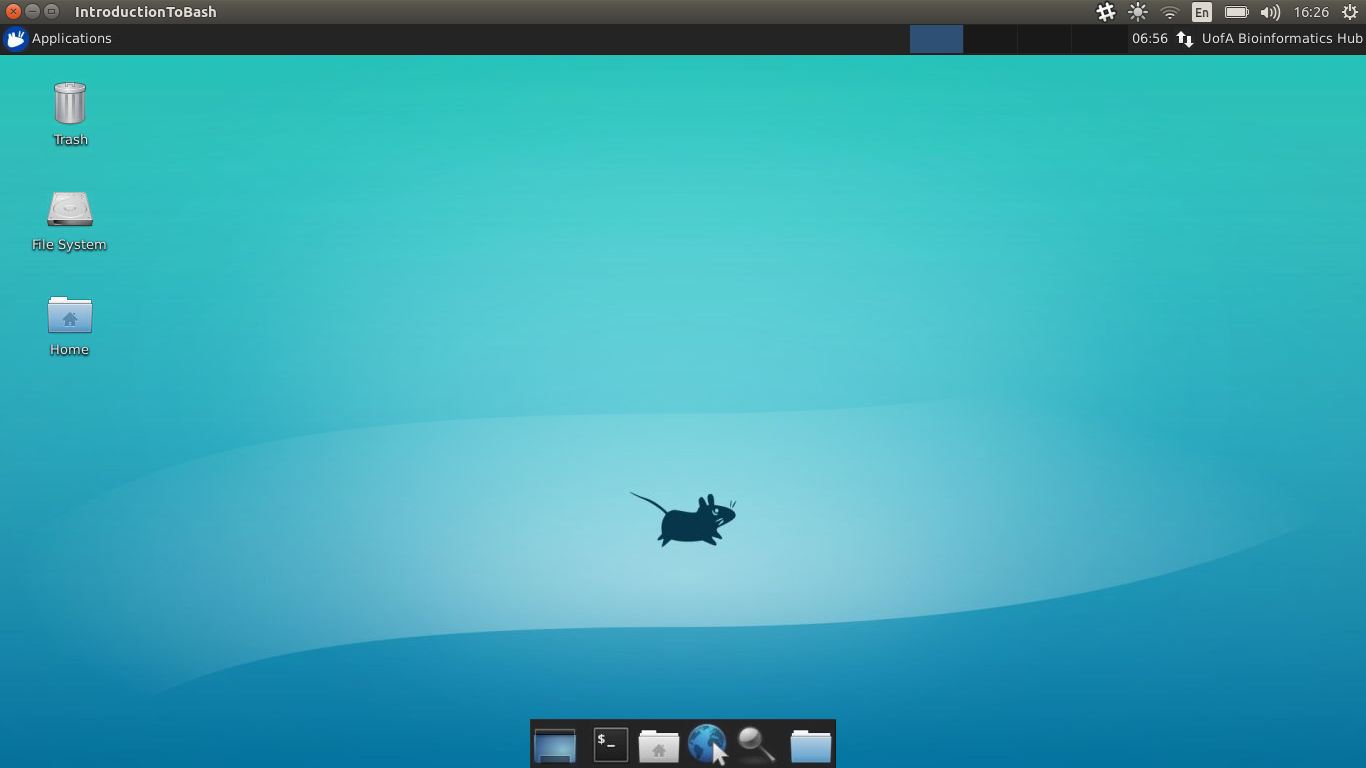
\includegraphics[width=0.9\linewidth]{images/xfceDesktop.png} 
	\caption{The VM desktop after logon with X2GO}
\end{figure}


\section{The Ubuntu Desktop}
\begin{note}
Now that you are connected, you will notice we are in a standard graphical environment.
The default Desktop in Ubuntu is Unity, but what we are seeing is one of the many alternatives, known as XFCE.
We are using this as it is the most simple for remote connections.
As many of us are used to seeing, there are click-able icons on the desktop, and drop-down menus. \\

Although we won't be using them today, Ubuntu has an built-in Office Suite of
programs which you can access from the \textit{Applications \textgreater Office} menu item.
This is where links can be found to open Document Viewer (a .pdf viewer), Libre Office Calc (Excel-like), Libre Office Writer (Word-like) \& other standard members of Office Program Suites. \\

The main interface we will be using today is the \texttt{terminal}which can be accessed from the set of icons at the bottom of you screen.
\textbf{Firefox} can also be accessed from the terminal using the command \texttt{firefox \&},  by clicking the \texttt{Web Browser} icon, or from the drop-down menu in the top left under the group \textit{Internet}.

\end{note}



%
% Start of modules
% Switch chapter styling to module
%
\chapterstyle{module}

%\clearpage
%\chapter{The Command Line}

%
% End of modules
% Switch back to normal workshop chapter styling
%
\chapterstyle{workshop}

\chapter{Space for Personal Notes or Feedback}
\clearpage

%
% Some empty ruled comments pages
%
\myruledpage{0cm}{1cm}
\myruledpage{0cm}{1cm}
\myruledpage{0cm}{1cm}
\myruledpage{0cm}{1cm}

\end{document}
